\documentclass[11pt,a4paper,]{article}
\usepackage{lmodern}

\usepackage{amssymb,amsmath}
\usepackage{ifxetex,ifluatex}
\usepackage{fixltx2e} % provides \textsubscript
\ifnum 0\ifxetex 1\fi\ifluatex 1\fi=0 % if pdftex
  \usepackage[T1]{fontenc}
  \usepackage[utf8]{inputenc}
\else % if luatex or xelatex
  \usepackage{unicode-math}
  \defaultfontfeatures{Ligatures=TeX,Scale=MatchLowercase}
\fi
% use upquote if available, for straight quotes in verbatim environments
\IfFileExists{upquote.sty}{\usepackage{upquote}}{}
% use microtype if available
\IfFileExists{microtype.sty}{%
\usepackage[]{microtype}
\UseMicrotypeSet[protrusion]{basicmath} % disable protrusion for tt fonts
}{}
\PassOptionsToPackage{hyphens}{url} % url is loaded by hyperref
\usepackage[unicode=true]{hyperref}
\hypersetup{
            pdftitle={Analysis on Gender Statictics},
            pdfborder={0 0 0},
            breaklinks=true}
\urlstyle{same}  % don't use monospace font for urls
\usepackage{geometry}
\geometry{a4paper, centering, text={16cm,24cm}}
\usepackage[style=authoryear-comp,]{biblatex}
\addbibresource{references.bib}
\usepackage{longtable,booktabs}
% Fix footnotes in tables (requires footnote package)
\IfFileExists{footnote.sty}{\usepackage{footnote}\makesavenoteenv{long table}}{}
\usepackage{graphicx,grffile}
\makeatletter
\def\maxwidth{\ifdim\Gin@nat@width>\linewidth\linewidth\else\Gin@nat@width\fi}
\def\maxheight{\ifdim\Gin@nat@height>\textheight\textheight\else\Gin@nat@height\fi}
\makeatother
% Scale images if necessary, so that they will not overflow the page
% margins by default, and it is still possible to overwrite the defaults
% using explicit options in \includegraphics[width, height, ...]{}
\setkeys{Gin}{width=\maxwidth,height=\maxheight,keepaspectratio}
\IfFileExists{parskip.sty}{%
\usepackage{parskip}
}{% else
\setlength{\parindent}{0pt}
\setlength{\parskip}{6pt plus 2pt minus 1pt}
}
\setlength{\emergencystretch}{3em}  % prevent overfull lines
\providecommand{\tightlist}{%
  \setlength{\itemsep}{0pt}\setlength{\parskip}{0pt}}
\setcounter{secnumdepth}{5}

% set default figure placement to htbp
\makeatletter
\def\fps@figure{htbp}
\makeatother


\title{Analysis on Gender Statictics}

%% MONASH STUFF

%% CAPTIONS
\RequirePackage{caption}
\DeclareCaptionStyle{italic}[justification=centering]
 {labelfont={bf},textfont={it},labelsep=colon}
\captionsetup[figure]{style=italic,format=hang,singlelinecheck=true}
\captionsetup[table]{style=italic,format=hang,singlelinecheck=true}


%% FONT
\RequirePackage{bera}
\RequirePackage[charter,expert,sfscaled]{mathdesign}
\RequirePackage{fontawesome}

%% HEADERS AND FOOTERS
\RequirePackage{fancyhdr}
\pagestyle{fancy}
\rfoot{\Large\sffamily\raisebox{-0.1cm}{\textbf{\thepage}}}
\makeatletter
\lhead{\textsf{\expandafter{\@title}}}
\makeatother
\rhead{}
\cfoot{}
\setlength{\headheight}{15pt}
\renewcommand{\headrulewidth}{0.4pt}
\renewcommand{\footrulewidth}{0.4pt}
\fancypagestyle{plain}{%
\fancyhf{} % clear all header and footer fields
\fancyfoot[C]{\sffamily\thepage} % except the center
\renewcommand{\headrulewidth}{0pt}
\renewcommand{\footrulewidth}{0pt}}

%% MATHS
\RequirePackage{bm,amsmath}
\allowdisplaybreaks

%% GRAPHICS
\RequirePackage{graphicx}
\setcounter{topnumber}{2}
\setcounter{bottomnumber}{2}
\setcounter{totalnumber}{4}
\renewcommand{\topfraction}{0.85}
\renewcommand{\bottomfraction}{0.85}
\renewcommand{\textfraction}{0.15}
\renewcommand{\floatpagefraction}{0.8}


%\RequirePackage[section]{placeins}

%% SECTION TITLES


%% SECTION TITLES (NEW: Changing sections and subsections color)
\RequirePackage[compact,sf,bf]{titlesec}
\titleformat*{\section}{\Large\sf\bfseries\color[rgb]{0.8, 0.7, 0.1 }}
\titleformat*{\subsection}{\large\sf\bfseries\color[rgb]{0.8, 0.7, 0.1 }}
\titleformat*{\subsubsection}{\sf\bfseries\color[rgb]{0.8, 0.7, 0.1 }}
\titlespacing{\section}{0pt}{2ex}{.5ex}
\titlespacing{\subsection}{0pt}{1.5ex}{0ex}
\titlespacing{\subsubsection}{0pt}{.5ex}{0ex}


%% TITLE PAGE
\def\Date{\number\day}
\def\Month{\ifcase\month\or
 January\or February\or March\or April\or May\or June\or
 July\or August\or September\or October\or November\or December\fi}
\def\Year{\number\year}

%% LINE AND PAGE BREAKING
\sloppy
\clubpenalty = 10000
\widowpenalty = 10000
\brokenpenalty = 10000
\RequirePackage{microtype}

%% PARAGRAPH BREAKS
\setlength{\parskip}{1.4ex}
\setlength{\parindent}{0em}

%% HYPERLINKS
\RequirePackage{xcolor} % Needed for links
\definecolor{darkblue}{rgb}{0,0,.6}
\RequirePackage{url}

\makeatletter
\@ifpackageloaded{hyperref}{}{\RequirePackage{hyperref}}
\makeatother
\hypersetup{
     citecolor=0 0 0,
     breaklinks=true,
     bookmarksopen=true,
     bookmarksnumbered=true,
     linkcolor=darkblue,
     urlcolor=blue,
     citecolor=darkblue,
     colorlinks=true}

\usepackage[showonlyrefs]{mathtools}
\usepackage[no-weekday]{eukdate}

%% BIBLIOGRAPHY

\makeatletter
\@ifpackageloaded{biblatex}{}{\usepackage[style=authoryear-comp, backend=biber, natbib=true]{biblatex}}
\makeatother
\ExecuteBibliographyOptions{bibencoding=utf8,minnames=1,maxnames=3, maxbibnames=99,dashed=false,terseinits=true,giveninits=true,uniquename=false,uniquelist=false,doi=false, isbn=false,url=true,sortcites=false}

\DeclareFieldFormat{url}{\texttt{\url{#1}}}
\DeclareFieldFormat[article]{pages}{#1}
\DeclareFieldFormat[inproceedings]{pages}{\lowercase{pp.}#1}
\DeclareFieldFormat[incollection]{pages}{\lowercase{pp.}#1}
\DeclareFieldFormat[article]{volume}{\mkbibbold{#1}}
\DeclareFieldFormat[article]{number}{\mkbibparens{#1}}
\DeclareFieldFormat[article]{title}{\MakeCapital{#1}}
\DeclareFieldFormat[article]{url}{}
%\DeclareFieldFormat[book]{url}{}
%\DeclareFieldFormat[inbook]{url}{}
%\DeclareFieldFormat[incollection]{url}{}
%\DeclareFieldFormat[inproceedings]{url}{}
\DeclareFieldFormat[inproceedings]{title}{#1}
\DeclareFieldFormat{shorthandwidth}{#1}
%\DeclareFieldFormat{extrayear}{}
% No dot before number of articles
\usepackage{xpatch}
\xpatchbibmacro{volume+number+eid}{\setunit*{\adddot}}{}{}{}
% Remove In: for an article.
\renewbibmacro{in:}{%
  \ifentrytype{article}{}{%
  \printtext{\bibstring{in}\intitlepunct}}}

\AtEveryBibitem{\clearfield{month}}
\AtEveryCitekey{\clearfield{month}}

\makeatletter
\DeclareDelimFormat[cbx@textcite]{nameyeardelim}{\addspace}
\makeatother

\author{\sf\Large\textbf{ Hsin Hsu}\\ {\sf\large 32195109\\[0.5cm]} \sf\Large\textbf{ Ratul Wadhwa}\\ {\sf\large 32055587\\[0.5cm]} \sf\Large\textbf{ Nelson Quintero}\\ {\sf\large 32254962\\[0.5cm]}}

\date{\sf\Date~\Month~\Year}
\makeatletter
\lfoot{\sf Hsu, Wadhwa, Quintero: \@date}
\makeatother


%%%% PAGE STYLE FOR FRONT PAGE OF REPORTS

\makeatletter
\def\organization#1{\gdef\@organization{#1}}
\def\telephone#1{\gdef\@telephone{#1}}
\def\email#1{\gdef\@email{#1}}
\makeatother
  \organization{Monash University}

  \def\name{Master of Business Analytics.}

  \telephone{(03) 9905 2478}

  \email{questions@company.com}                 %NEW: New email addresss

\def\webaddress{\url{http://company.com/stats/consulting/}} %NEW: URl
\def\abn{12 377 614 630}                                    % NEW: ABN
\def\logo{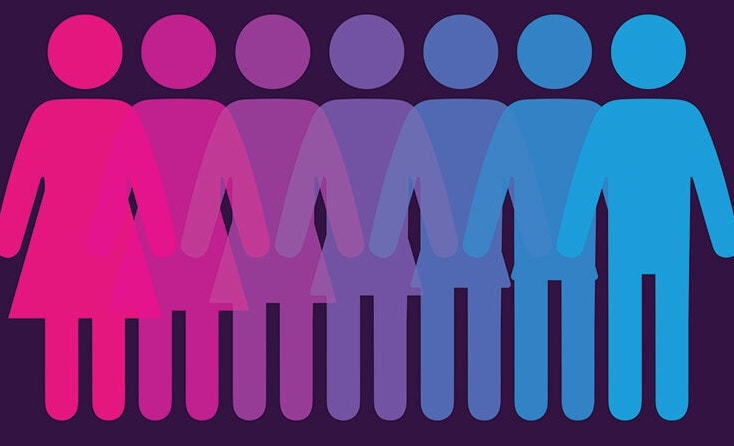
\includegraphics[width=6cm]{Figures/logo}}  %NEW: Changing logo
\def\extraspace{\vspace*{1.6cm}}
\makeatletter
\def\contactdetails{\faicon{phone} & \@telephone \\
                    \faicon{envelope} & \@email}
\makeatother

%%%% FRONT PAGE OF REPORTS

\def\reporttype{Report for}

\long\def\front#1#2#3{
\newpage
\begin{singlespacing}
\thispagestyle{empty}
\vspace*{-1.4cm}
\hspace*{-1.4cm}
\hbox to 16cm{
  \hbox to 6.5cm{\vbox to 14cm{\vbox to 25cm{
    \logo
    \vfill
    \parbox{6.3cm}{\raggedright
      \sf\color[rgb]{0.8, 0.7, 0.1 }    % NEW color 
      {\large\textbf{\name}}\par
      \vspace{.7cm}
      \tabcolsep=0.12cm\sf\small
      \begin{tabular}{@{}ll@{}}\contactdetails
      \end{tabular}
      \vspace*{0.3cm}\par
      ABN: \abn\par
    }
  }\vss}\hss}
  \hspace*{0.2cm}
  \hbox to 1cm{\vbox to 14cm{\rule{4pt}{26.8cm}\vss}\hss\hfill}  %NEW: Thicker line
  \hbox to 10cm{\vbox to 14cm{\vbox to 25cm{   
      \vspace*{3cm}\sf\raggedright
      \parbox{11cm}{\sf\raggedright\baselineskip=1.2cm
         \fontsize{24.88}{30}\color[rgb]{0, 0.29, 0.55}\sf\textbf{#1}}   % NEW: title color blue
      \par
      \vfill
      \large
      \vbox{\parskip=0.8cm #2}\par
      \vspace*{2cm}\par
      \reporttype\\[0.3cm]
      \hbox{#3}%\\[2cm]\
      \vspace*{1cm}
      {\large\sf\textbf{\Date~\Month~\Year}}
   }\vss}
  }}
\end{singlespacing}
\newpage
}

\makeatletter
\def\titlepage{\front{\expandafter{\@title}}{\@author}{\@organization}}
\makeatother

\usepackage{setspace}
\setstretch{1.5}

\usepackage{float}
\let\origfigure\figure
\let\endorigfigure\endfigure
\renewenvironment{figure}[1][2] {
    \expandafter\origfigure\expandafter[H]
} {
    \endorigfigure
}
%% Any special functions or other packages can be loaded here.
\usepackage{float}
\usepackage{booktabs}
\usepackage{longtable}
\usepackage{array}
\usepackage{multirow}
\usepackage{wrapfig}
\usepackage{colortbl}
\usepackage{pdflscape}
\usepackage{tabu}
\usepackage{threeparttable}
\usepackage{threeparttablex}
\usepackage[normalem]{ulem}
\usepackage{makecell}
\usepackage{xcolor}


\begin{document}
\titlepage

{
\setcounter{tocdepth}{2}
\tableofcontents
}
\clearpage

\hypertarget{introduction}{%
\section{Introduction}\label{introduction}}

The \href{https://data.worldbank.org/}{World Bank Data Group} coordinates statistical and data work and maintains a number of macro, financial and sector databases. The group is guided by professional standards in the collection, compilation and dissemination of data to ensure that all data users can have confidence in the quality and integrity of the data produced.

Gender inequality remains a major barrier to human development. Girls and women have made major strides since 1990, but they have not yet gained gender equity. Women who want to work have a harder time finding a job than men. This problem is particularly marked in developing countries where unemployment rates for women is more than that of developed countries.

Hence, the primary analysis of our report is to compare and contrast the gender statistic in developed countries like \textbf{United States \& France} and developing countries like \textbf{Colombia and Egypt} from the years 2010 to 2019 on various factors like:

\begin{itemize}
\item
  The section 1 of the report contains comparison of \textbf{inflation, gender distribution for labour force and life expectancy} in various countries.
\item
  The section 2 of the report contains gender work flow distribution and \textbf{gender work flow comparison in various sectors like agriculture, industry and service}
\item
  The section 3 of the report contains the analysis on the total unemployment difference between males and females and \textbf{analysis on the basis of qualifications in developed and developing countries.}
\end{itemize}

\clearpage

\hypertarget{analysis}{%
\section{Analysis}\label{analysis}}

\section*{Section 1}

\hypertarget{inflation}{%
\subsection{Inflation}\label{inflation}}

\begin{verbatim}
## [[1]]
\end{verbatim}

\begin{figure}
\centering
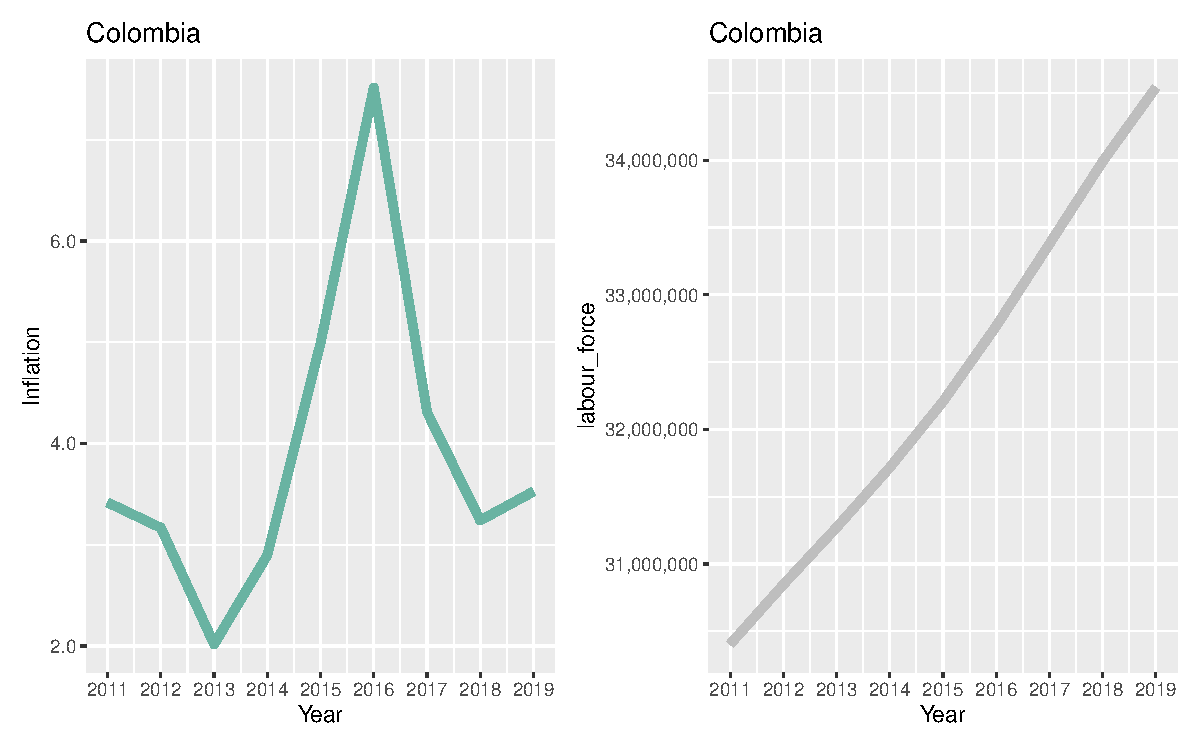
\includegraphics{The_Outsiders_5513_files/figure-latex/A1-1.pdf}
\caption{\label{fig:A1-1}Inflation vs Labour force}
\end{figure}

\begin{verbatim}
## 
## [[2]]
\end{verbatim}

\begin{figure}
\centering
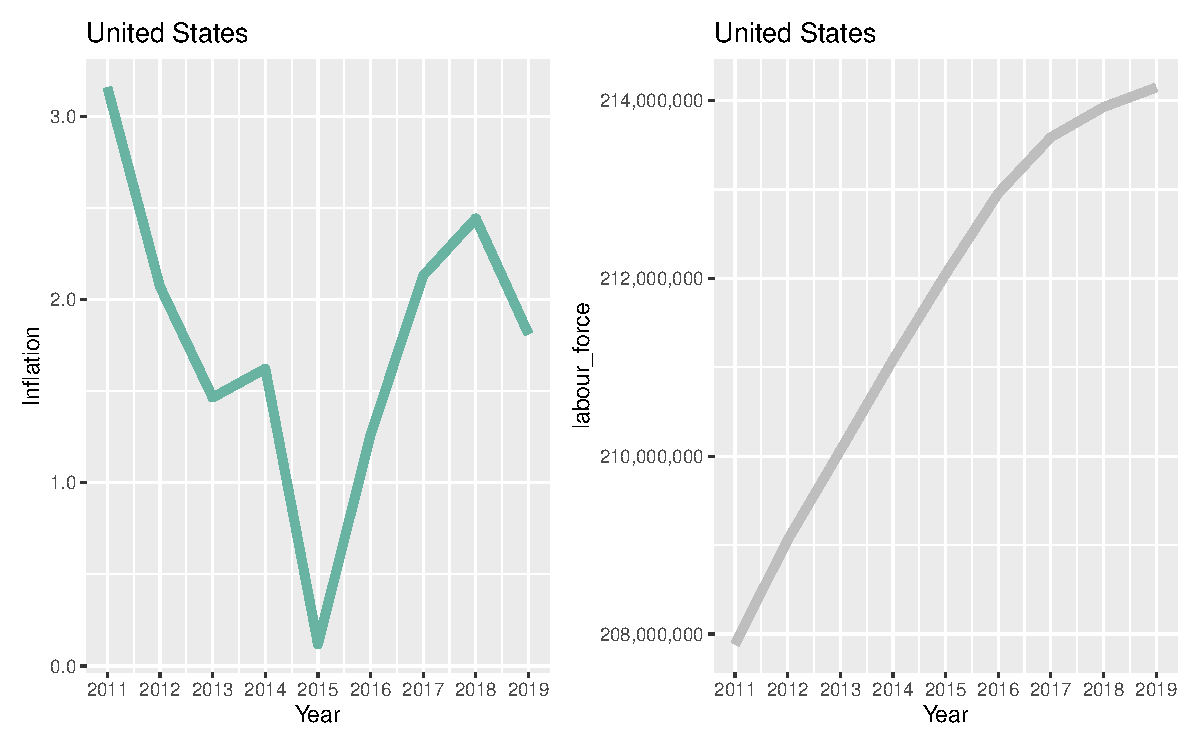
\includegraphics{The_Outsiders_5513_files/figure-latex/A1-2.pdf}
\caption{\label{fig:A1-2}Inflation vs Labour force}
\end{figure}

\begin{verbatim}
## 
## [[3]]
\end{verbatim}

\begin{figure}
\centering
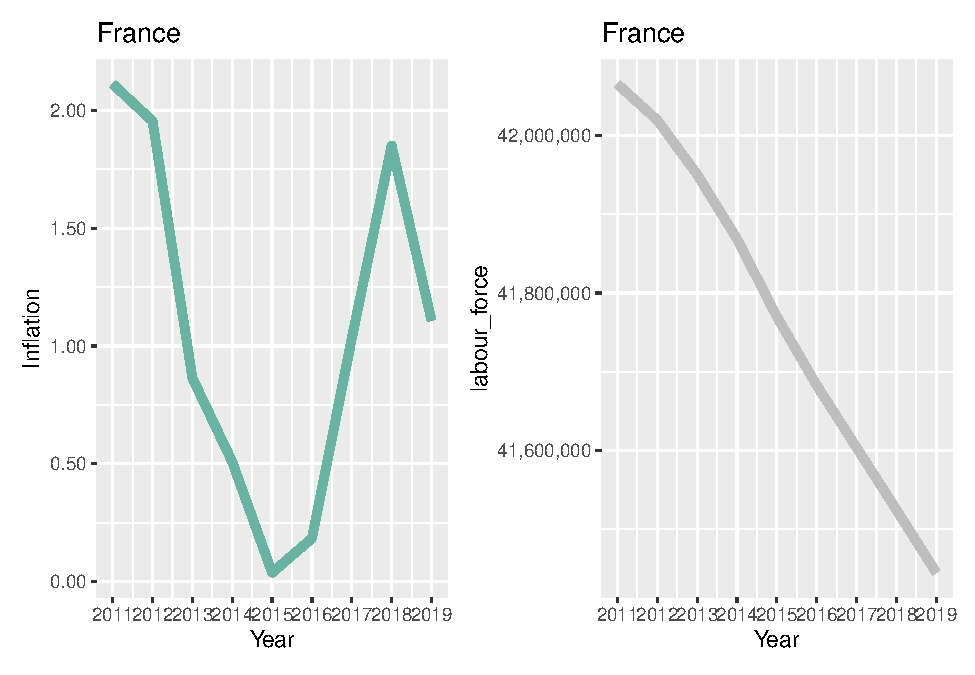
\includegraphics{The_Outsiders_5513_files/figure-latex/A1-3.pdf}
\caption{\label{fig:A1-3}Inflation vs Labour force}
\end{figure}

\begin{verbatim}
## 
## [[4]]
\end{verbatim}

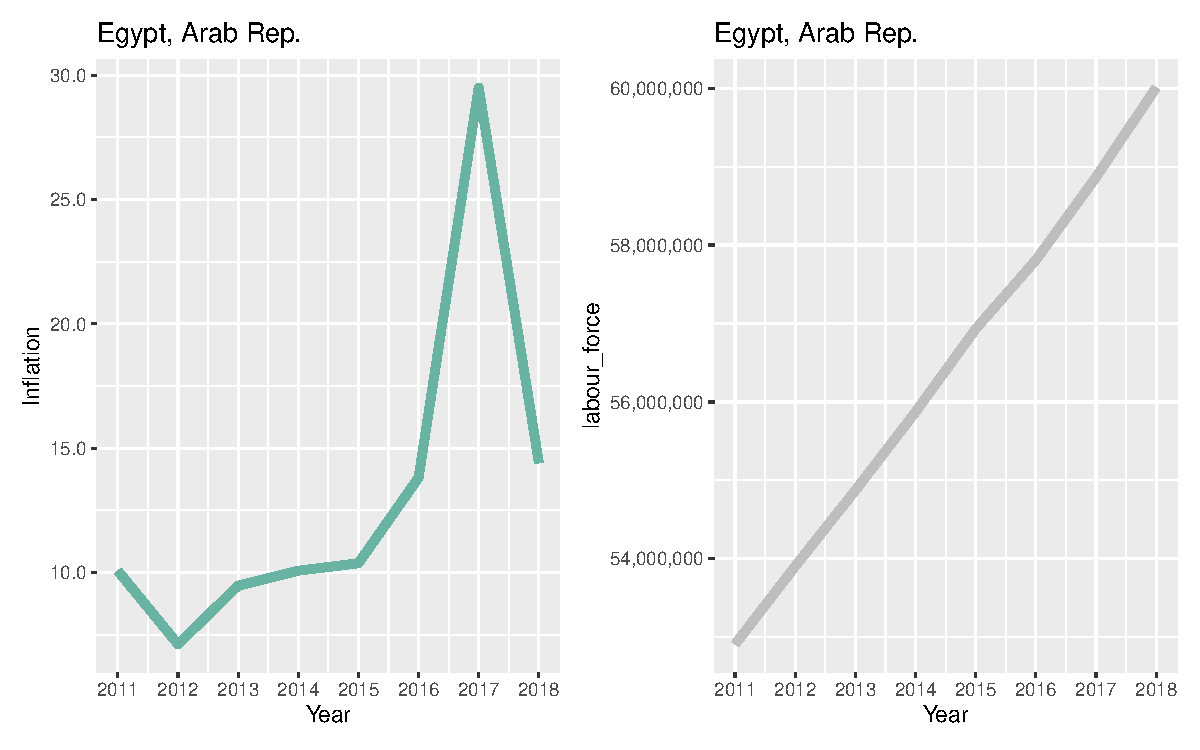
\includegraphics{The_Outsiders_5513_files/figure-latex/A1-4.pdf}
According to the figures above, developed countries such as United States and France both have the lowest inflation rate in 2015. This is because in 2015, the crude oil price collapsed. \autocite{stocker}, and the global economy has not recovered from the GFC yet \autocite{inflation1}.

Moreover, low inflation rate does not mean the currency is more valuable. On the contrary, it signals demand for goods and services is lower than expected and will then result in recession and the an increase in unemployment \autocite{inflation2}.

Additionally, developed countries usually have more stable inflation rate than developing countries. This is to keep the economy and the currency stable.

\begin{table}

\caption{\label{tab:A2}Inflation and the labour force in 2015}
\centering
\begin{tabular}[t]{l|r|r|r}
\hline
Country Name & Year & Inflation & labour\_force\\
\hline
Colombia & 2015 & 4.9902343 & 32207438\\
\hline
United States & 2015 & 0.1186271 & 212046898\\
\hline
France & 2015 & 0.0375144 & 41770007\\
\hline
Egypt, Arab Rep. & 2015 & 10.3704903 & 56930104\\
\hline
\end{tabular}
\end{table}

Table \ref{tab:A2} shows the 2015 inflation rate.

\hypertarget{gender-distribution-for-labour-force}{%
\subsection{Gender distribution for labour force}\label{gender-distribution-for-labour-force}}

Moreover, the labour force in each country is increasing but decreasing in France. We will take a deeper look in the employment and unemployment in the following sections and try to conclude why the labour force for France is decreasing.

Let's also look at the gender distribution in the labour force.

\begin{figure}
\centering
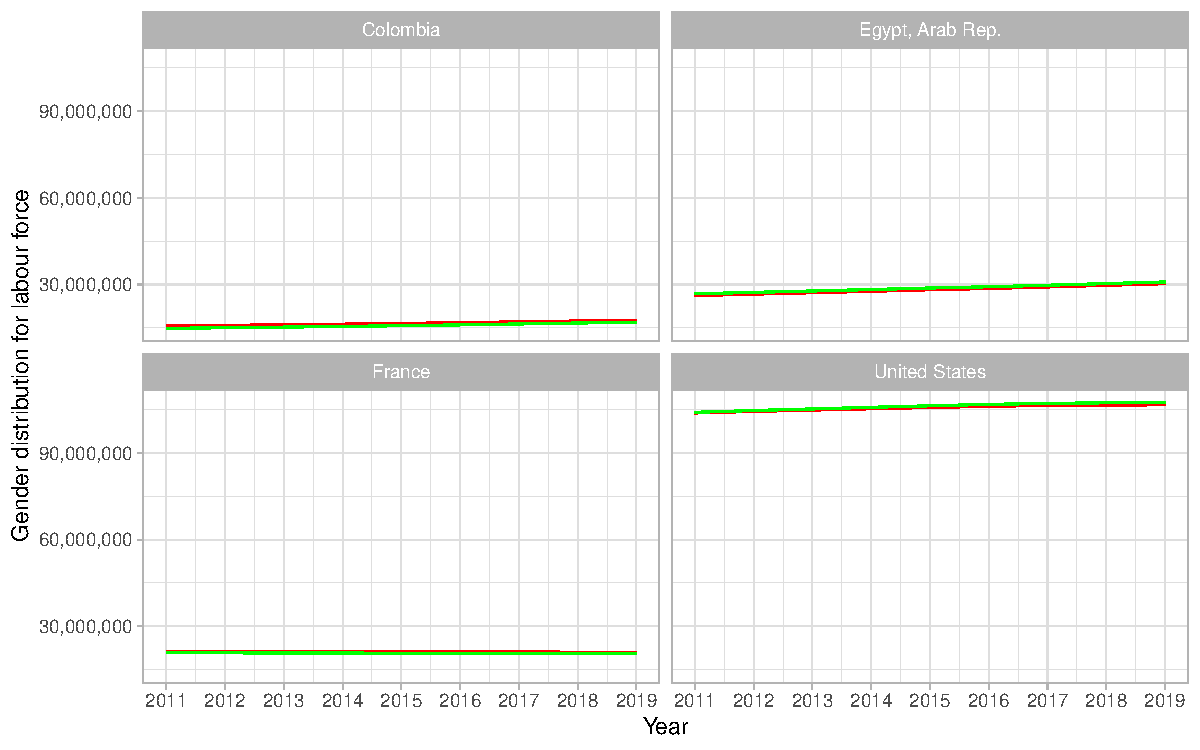
\includegraphics{The_Outsiders_5513_files/figure-latex/A3-1.pdf}
\caption{\label{fig:A3}Gender distribution for labour force}
\end{figure}

Figure \ref{fig:A3} shows the lines for female labour force and the male labour force are almost overlapped with each other, meaning the gender distribution for labour force is fairly equal in these countries.

\hypertarget{life-expectancy-for-female-and-male-at-birth}{%
\subsection{Life expectancy for female and male at birth}\label{life-expectancy-for-female-and-male-at-birth}}

\begin{figure}
\centering
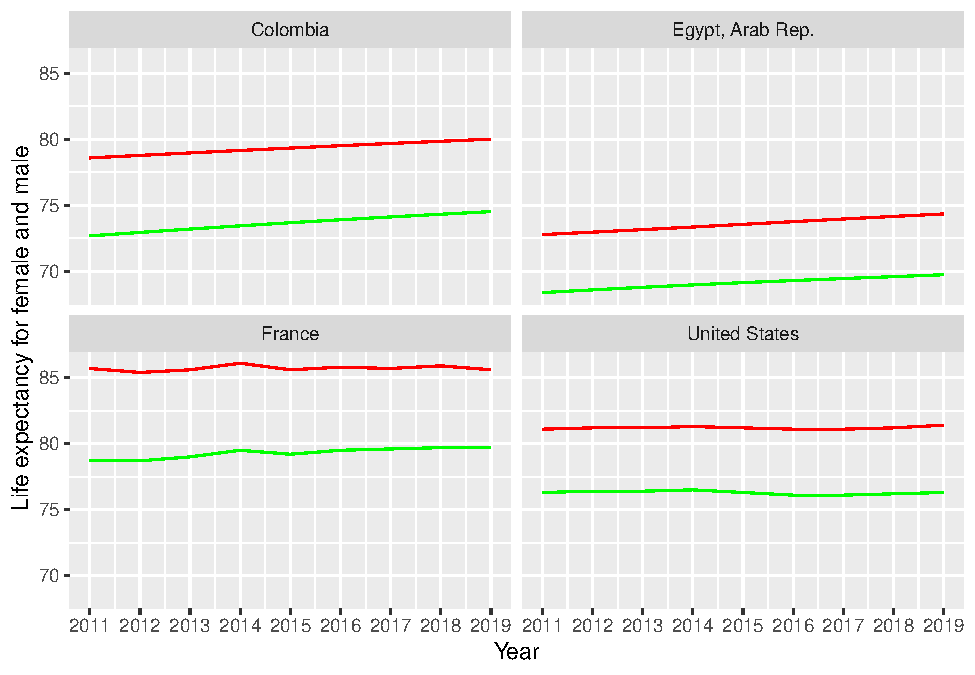
\includegraphics{The_Outsiders_5513_files/figure-latex/A4-1.pdf}
\caption{\label{fig:A4}Life expectancy for female and male at birth}
\end{figure}

Figure \ref{fig:A4} shows the life expectancy for female is obviously higher than male. More interestingly, US and France are having a stable life expectancy from 2011 til 2019, while in Egypt and Colombia, the life expectancy for both genders is increasing.

\clearpage

\section*{Section 2}

\hypertarget{employment-analysis-by-country}{%
\subsection{Employment Analysis by Country}\label{employment-analysis-by-country}}

The core analysis of this report is to analyze the different workforce distribution among high and low income countries and the gender distribution inside them. High income countries such as United States and France and low income such as Colombia and Egypt were taken into account to evaluate the labor force condition and the general trends of the citizens performing jobs in agriculture, industry and services jobs.

Having a closer look to the data, the distribution in the job market according to the gender and country it is taking part in, tends to variate according to the economy of each country. High income countries such as United States or France manages a similar trend in every industry according to the gender. But also, it can be seen that the rates are different compared to the low income countries.

\hypertarget{high-income-countries-workforce}{%
\subsection{High Income Countries Workforce}\label{high-income-countries-workforce}}

The higher income countries have, the higher participation in services by males. On the other hand, there is lower concentration in the participation of female in industries that are considered ``Masculine'' for the time being, agriculture and industry.

For high income countries the similarity in the allocation of workforce among the studies industries is surprisingly similar. in the figure \ref{fig:highinc} USA and France have an average of 67\% of male workforce, also, have a similar percentage by 2019 in industry of 30\% and in agriculture of 4\%.

Generally, females are on top of the chart with about 90\% working in services, and with similar rates for agriculture and industry of 1\% and 9\% respectively.

\begin{figure}
\centering
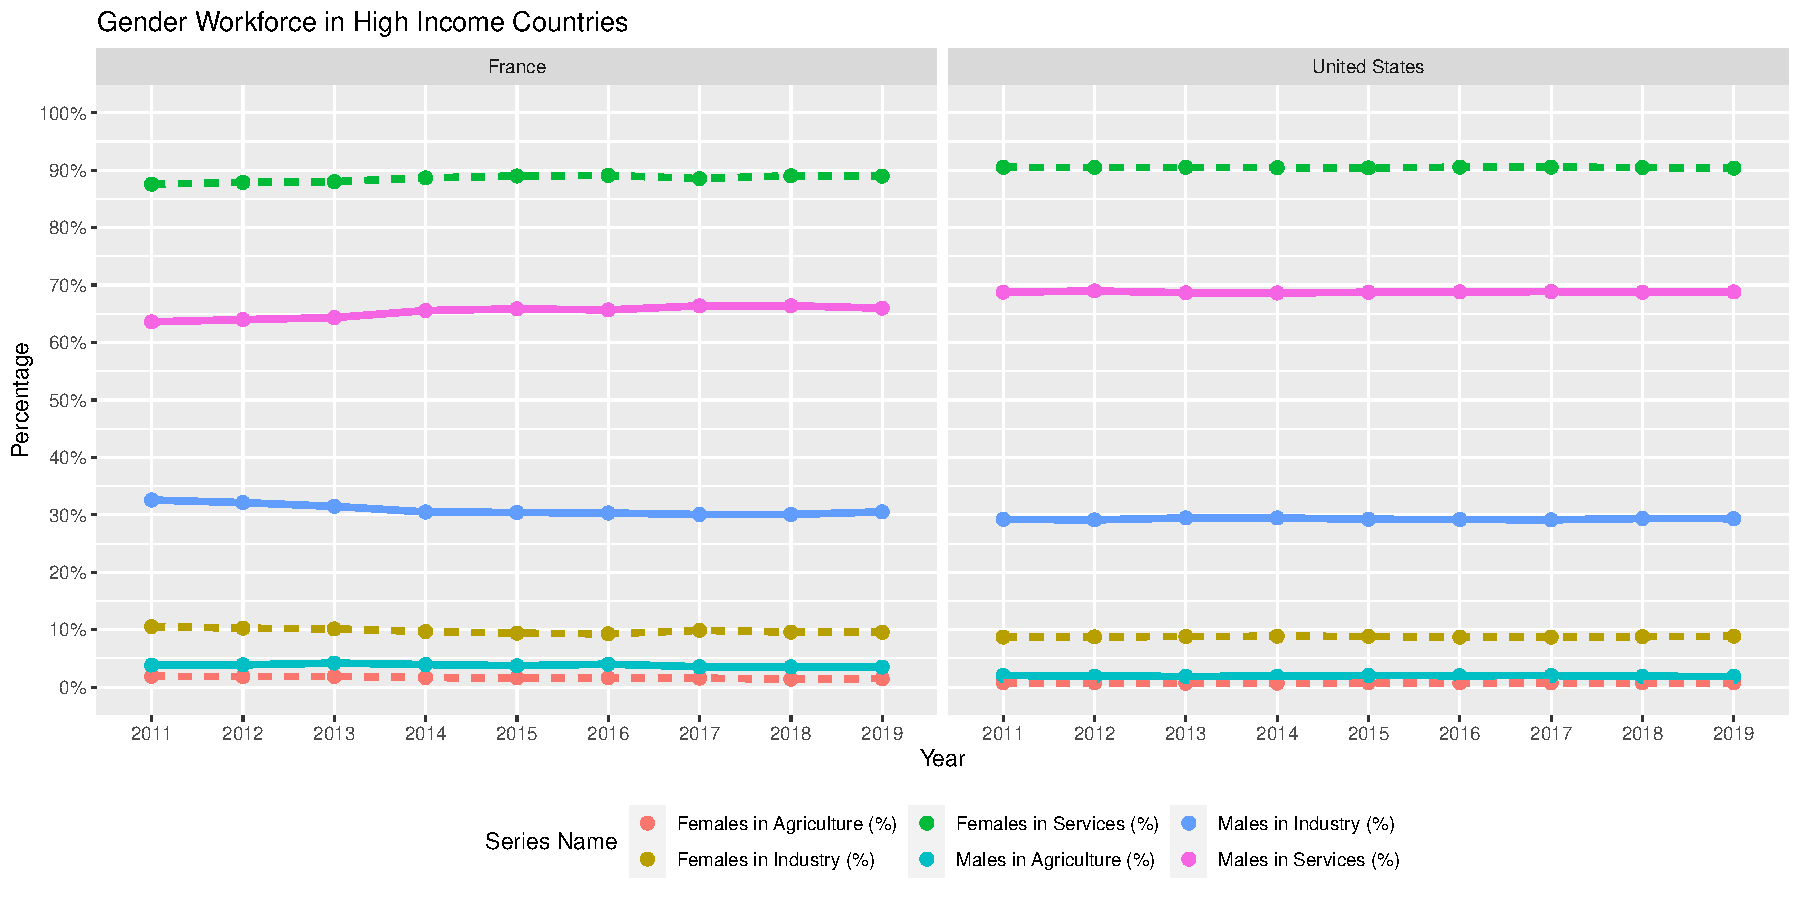
\includegraphics{The_Outsiders_5513_files/figure-latex/highinc-1.pdf}
\caption{\label{fig:highinc}High Income Countries Workforce}
\end{figure}

\hypertarget{low-income-countries-workforce}{%
\subsection{Low Income Countries Workforce}\label{low-income-countries-workforce}}

Males in the job market for low income countries keep similar trends for the jobs in agriculture. In 2019, in Colombia and Egypt got in average 25\% of male participation. In industry, Colombia and Egypt have a notorious difference of 25\% and 32\% respectively.

In the case of females, they keep an average from 10\% to 20\% in ``Masculine'' jobs, as per in services, they keep from 50\% to 80\%. Egypt had a huge decline in the agricultural jobs for females from a 43\% to 21\%. It is remarkable this variation along the previous 9 years as well as that the woman workforce seemed to move in the same rate to the services industry as seen in the figure \ref{fig:lowinc} below. \autocite{WDAgriculture}

\begin{figure}
\centering
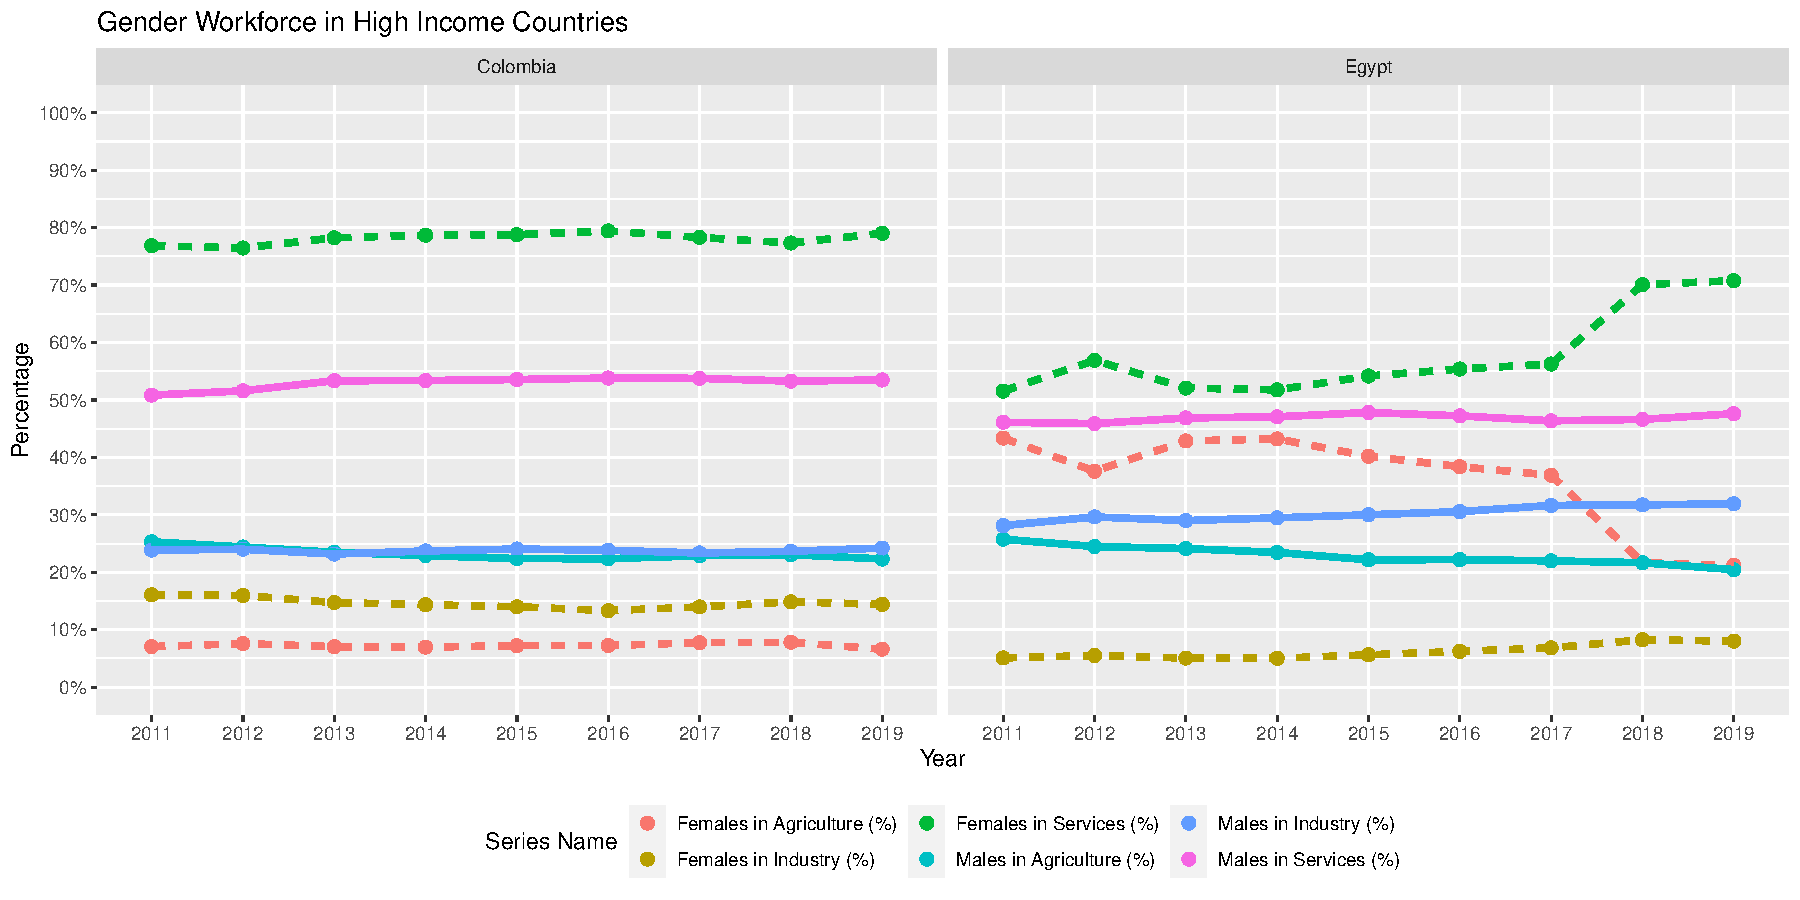
\includegraphics{The_Outsiders_5513_files/figure-latex/lowinc-1.pdf}
\caption{\label{fig:lowinc}Low Income Countries Workforce}
\end{figure}

\hypertarget{gender-workforce-distribution-by-country}{%
\subsection{Gender Workforce Distribution by Country}\label{gender-workforce-distribution-by-country}}

As seen in the current analysis the economical capacity of the countries can infer in the workforce distribution. In a general view of the selected samples, females have in all of them the highest rate of employment in services as well as the lowest in agriculture, this does not apply in Egypt but the current trend is showing that there is a moving out of that industry.

Similarly, males have the highest level of employment in services, but they keep leading the industry and agricultural workforce. It is noticeable that if a country is wealthy, there is a higher level of participation of females in service jobs compared to low income countries. On the other hand, despite the income level of the country males keep the same percentage among the countries. See figure \ref{fig:allcountries}.

\begin{figure}
\centering
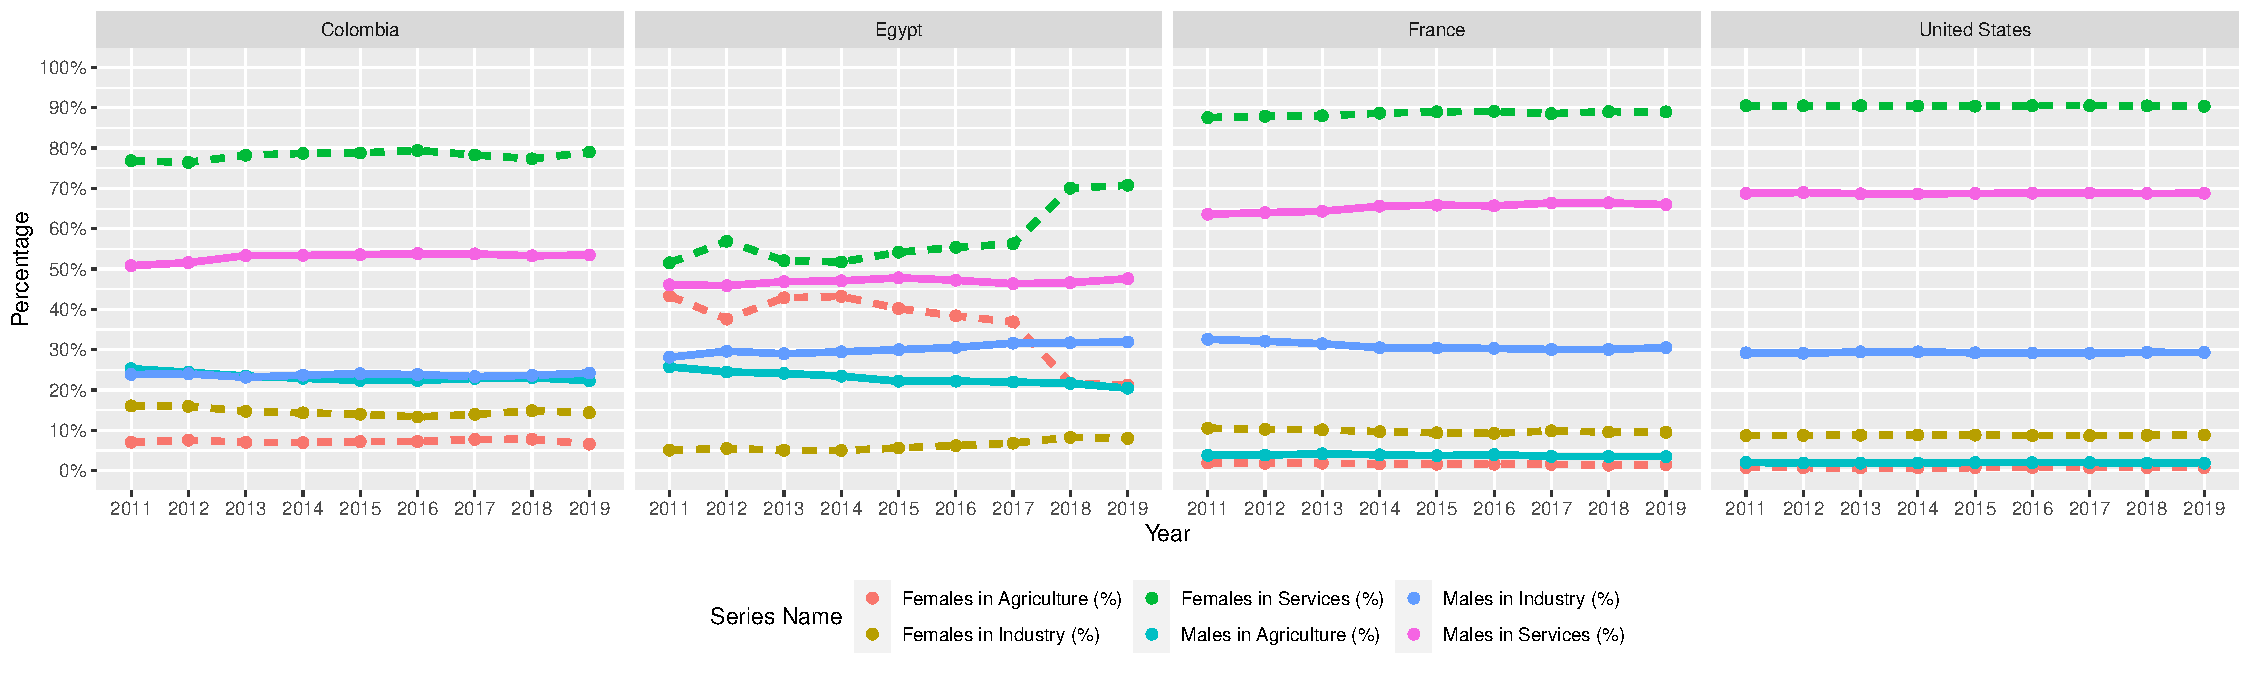
\includegraphics{The_Outsiders_5513_files/figure-latex/allcountries-1.pdf}
\caption{\label{fig:allcountries}Gender Workforce Distribution by Country}
\end{figure}

\hypertarget{gender-workforce-comparison-by-industry.}{%
\subsection{Gender Workforce Comparison by Industry.}\label{gender-workforce-comparison-by-industry.}}

From other point of view and analyzing the variables across all the countries it can be seen that the genders maintain a similar level of employment according to the selected industries.

\hypertarget{female-and-male-employment-in-agriculture.}{%
\subsection{Female and Male Employment in Agriculture.}\label{female-and-male-employment-in-agriculture.}}

in the figure \ref{fig:agriculture} women keep the lowest participation in agriculture and industry jobs in the selected countries except Egypt which have had a decrease around of 50\% during the past 9 years, keeping lowest rates compared to male results. The level of jobs have been steady for males and females during the analyzed years.

\begin{figure}
\centering
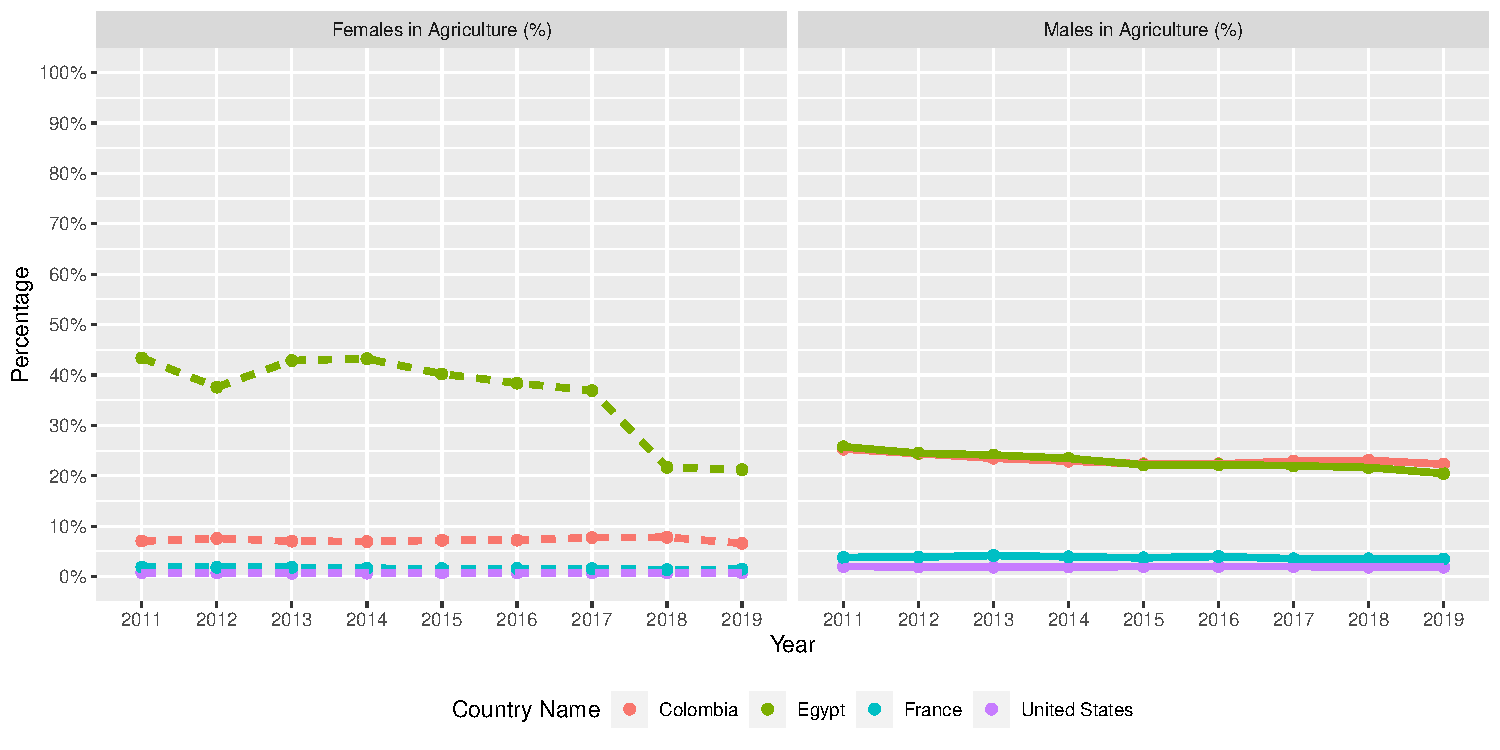
\includegraphics{The_Outsiders_5513_files/figure-latex/agriculture-1.pdf}
\caption{\label{fig:agriculture}Female and Male Employment in Agriculture}
\end{figure}

\hypertarget{female-and-male-employment-in-industry.}{%
\subsection{Female and Male Employment in Industry.}\label{female-and-male-employment-in-industry.}}

In the case of industry jobs, male keep a highest rate compared to female across the analyzed countries. In 2019 the number of female rose by 5\% in Egypt, while in Colombia decreased by 2\% and in USA and France maintained the same levels.

In the case of males, all the countries maintained about the same levels since 2011 as seen in the figure \ref{fig:industry}.

\begin{figure}
\centering
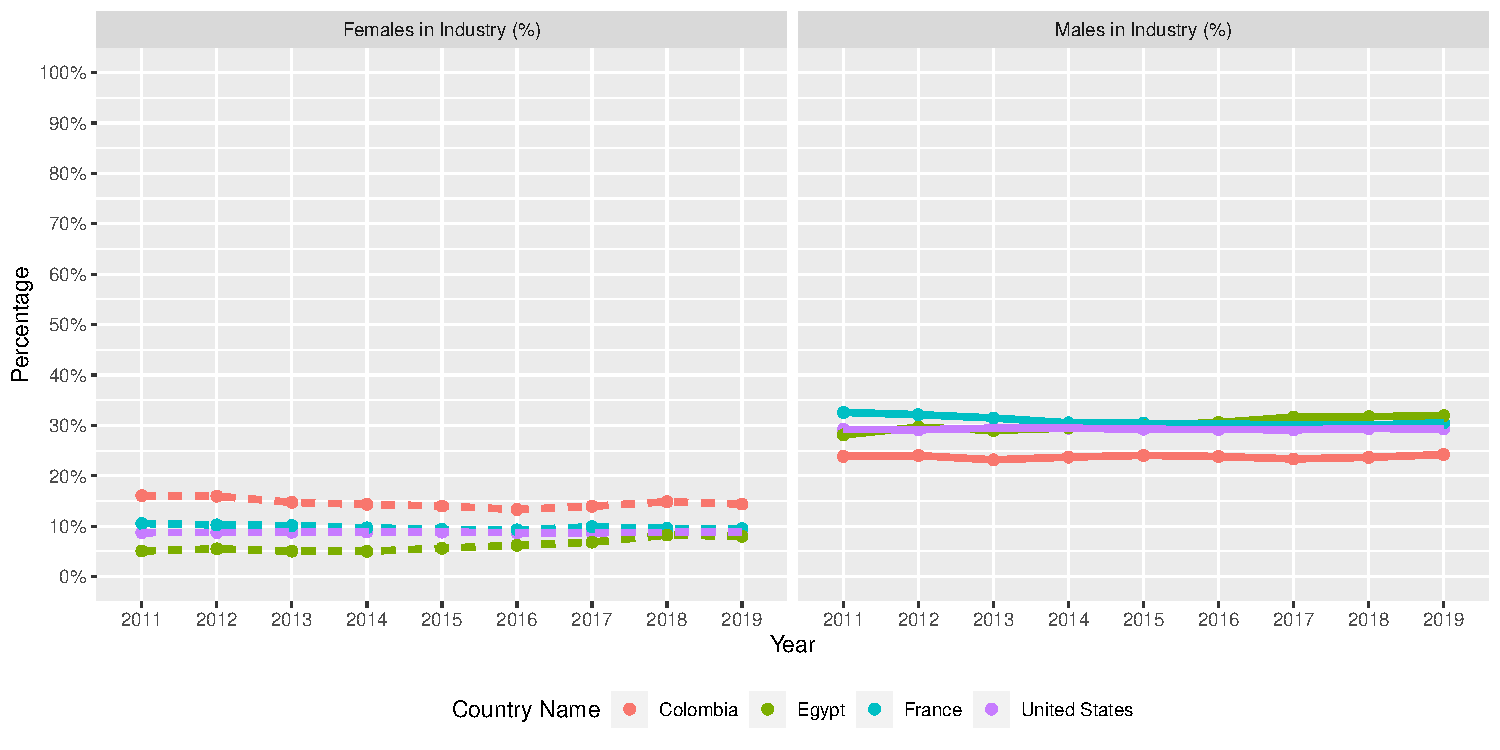
\includegraphics{The_Outsiders_5513_files/figure-latex/industry-1.pdf}
\caption{\label{fig:industry}Female and Male Employment in Industry}
\end{figure}

\hypertarget{female-and-male-employment-in-services.}{%
\subsection{Female and Male Employment in Services.}\label{female-and-male-employment-in-services.}}

Female have a highest participation in the services sector compared to males and across all the industries.

In general, all the countries kept the same average levels since 2011 and they are in a similar range despite the income level of the country. But, Egypt has an interesting variation of the the jobs allocation. In this case, females in services have rose over 30\% in the last years, maintaining the leading over their male peers. In this Industry Egypt has the lowest of people, but the trend keeps a future positive path as well as France. See figure \ref{fig:services}.

\begin{figure}
\centering
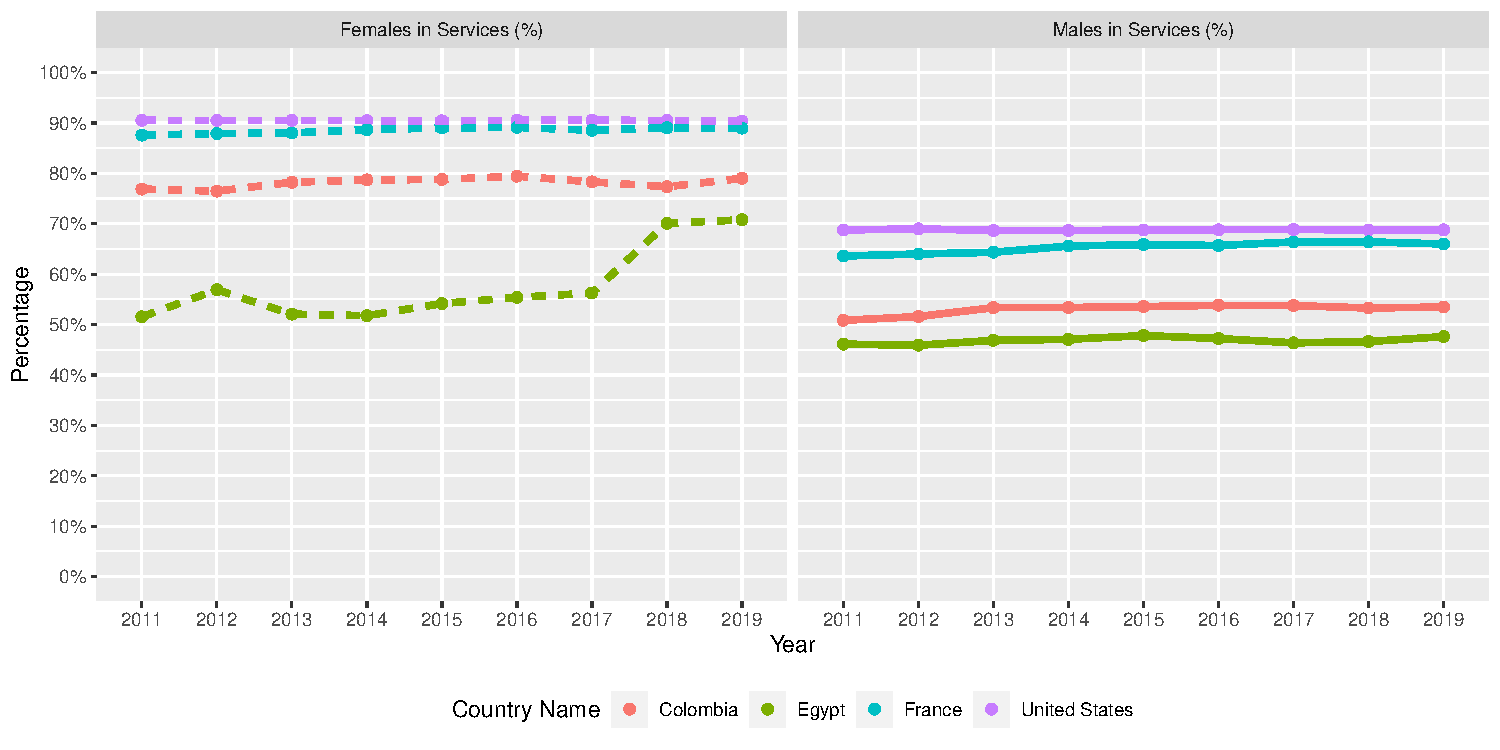
\includegraphics{The_Outsiders_5513_files/figure-latex/services-1.pdf}
\caption{\label{fig:services}Female and Male Employment in Services}
\end{figure}

\hypertarget{gender-workforce-by-industry}{%
\subsection{Gender Workforce by Industry}\label{gender-workforce-by-industry}}

In summary, females across all countries have lower levels than male occupations in agriculture and industry. On the other hand females have the lead in the services job market, the most notorious case of growth in this industry was Egypt that in 2019 the percentage of females in this industry was 71\%.

\begin{figure}
\centering
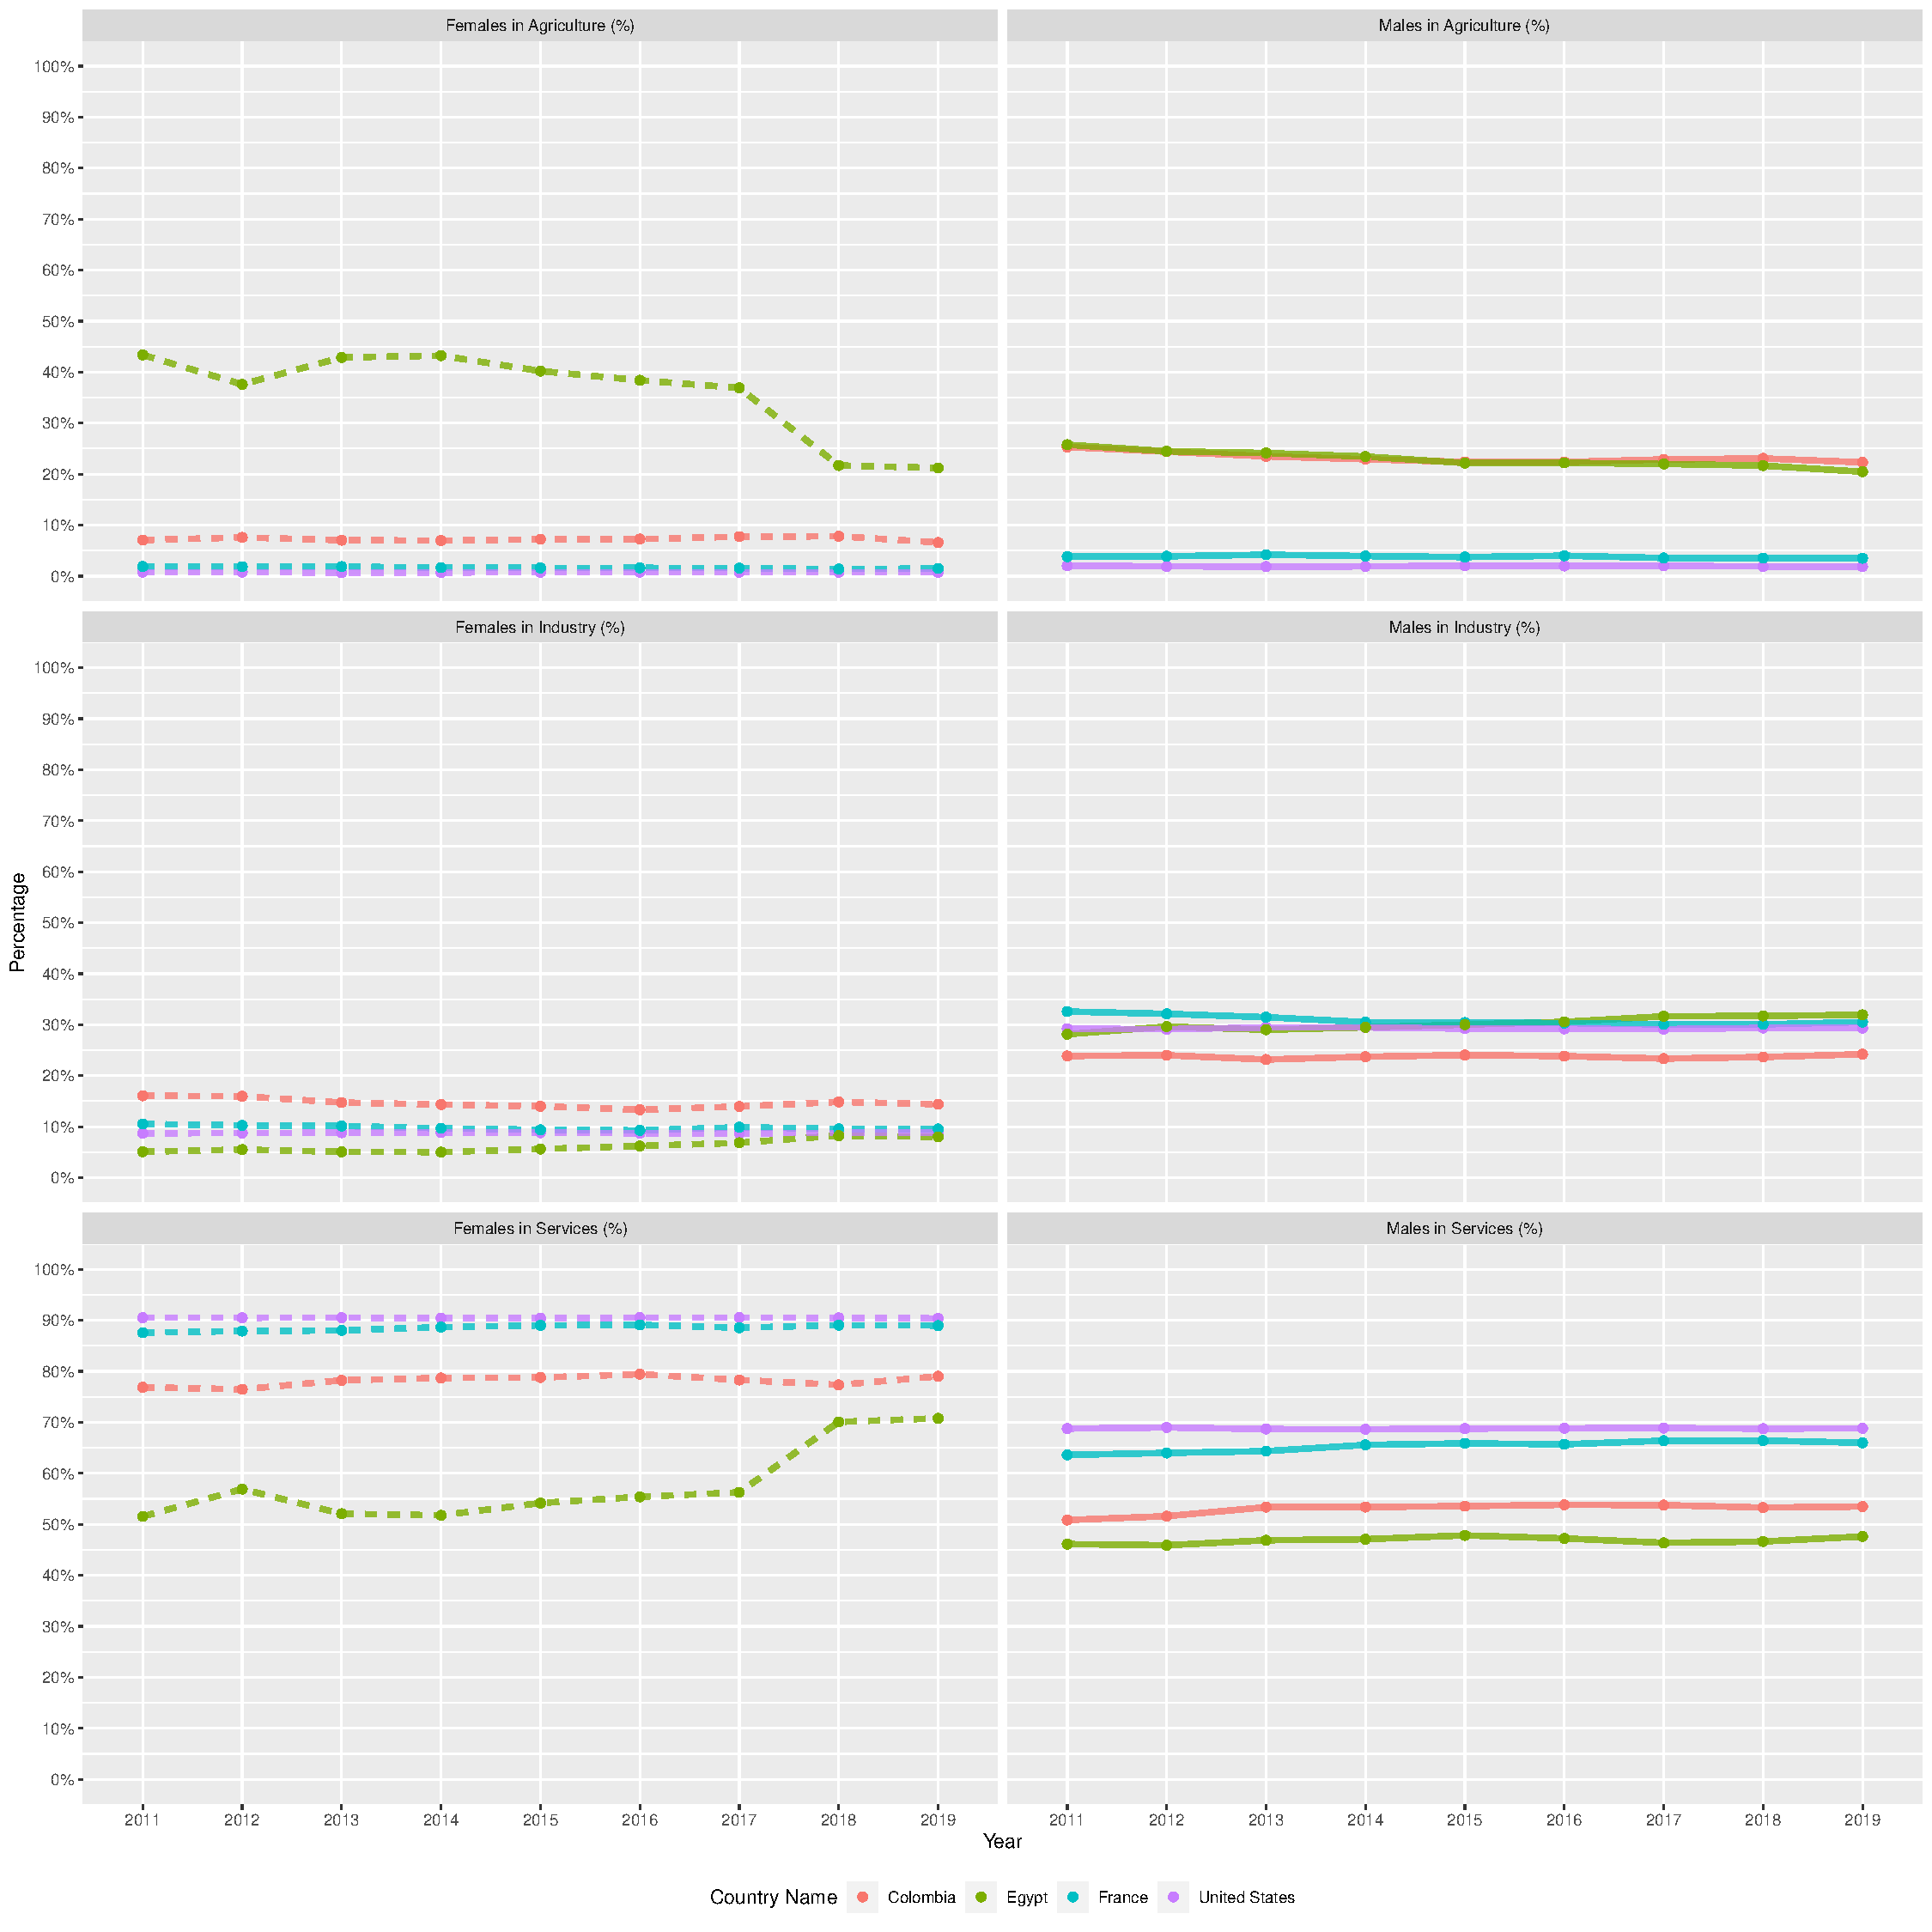
\includegraphics{The_Outsiders_5513_files/figure-latex/allvars-1.pdf}
\caption{\label{fig:allvars}Gender Workforce by Industry}
\end{figure}

\clearpage

\section*{Section 3}

\hypertarget{analysis-on-total-unemployed-males-and-females-in-developed-and-developing-countries}{%
\subsection{Analysis on total unemployed males and females in developed and developing countries}\label{analysis-on-total-unemployed-males-and-females-in-developed-and-developing-countries}}

\textbf{United States \& France}

\begin{table}[H]

\caption{\label{tab:tabref}Unemployed percentage of males and females in Developed countries}
\centering
\begin{tabular}[t]{l|l|r|r}
\hline
Country Name & Year & Unemployed\_F & Unemployed\_M\\
\hline
France & 2011 & 9.12 & 8.530000\\
\hline
France & 2012 & 9.36 & 9.440000\\
\hline
France & 2013 & 9.79 & 10.040000\\
\hline
France & 2014 & 10.03 & 10.540000\\
\hline
France & 2015 & 9.91 & 10.770001\\
\hline
France & 2016 & 9.84 & 10.220000\\
\hline
France & 2017 & 9.37 & 9.440000\\
\hline
France & 2018 & 9.05 & 8.990000\\
\hline
France & 2019 & 8.38 & 8.500000\\
\hline
United States & 2011 & 8.46 & 9.370000\\
\hline
United States & 2012 & 7.89 & 8.229999\\
\hline
United States & 2013 & 7.08 & 7.640000\\
\hline
United States & 2014 & 6.06 & 6.260000\\
\hline
\cellcolor{red}{\textcolor{white}{\textbf{United States}}} & \cellcolor{red}{\textcolor{white}{\textbf{2015}}} & \cellcolor{red}{\textcolor{white}{\textbf{5.18}}} & \cellcolor{red}{\textcolor{white}{\textbf{5.370000}}}\\
\hline
United States & 2016 & 4.79 & 4.940000\\
\hline
United States & 2017 & 4.31 & 4.400000\\
\hline
United States & 2018 & 3.84 & 3.950000\\
\hline
United States & 2019 & 3.61 & 3.720000\\
\hline
\end{tabular}
\end{table}

\textbf{Colombia \& Egypt, Arab Rep.}

\begin{table}[H]

\caption{\label{tab:tabref1}Unemployed percentage of males and females in Developing countries}
\centering
\begin{tabular}[t]{l|l|r|r}
\hline
Country Name & Year & Unemployed\_F & Unemployed\_M\\
\hline
Colombia & 2011 & 13.10 & 7.910000\\
\hline
Colombia & 2012 & 12.66 & 7.550000\\
\hline
Colombia & 2013 & 11.67 & 7.070000\\
\hline
Colombia & 2014 & 11.03 & 6.720000\\
\hline
Colombia & 2015 & 10.84 & 6.360000\\
\hline
Colombia & 2016 & 11.21 & 6.780000\\
\hline
Colombia & 2017 & 11.51 & 6.870000\\
\hline
Colombia & 2018 & 11.79 & 7.090000\\
\hline
Colombia & 2019 & 12.75 & 7.880000\\
\hline
Egypt, Arab Rep. & 2011 & 22.44 & 8.770001\\
\hline
Egypt, Arab Rep. & 2012 & 24.01 & 9.229999\\
\hline
Egypt, Arab Rep. & 2013 & 24.17 & 9.800000\\
\hline
Egypt, Arab Rep. & 2014 & 24.00 & 9.729999\\
\hline
\cellcolor{red}{\textcolor{white}{\textbf{Egypt, Arab Rep.}}} & \cellcolor{red}{\textcolor{white}{\textbf{2015}}} & \cellcolor{red}{\textcolor{white}{\textbf{24.81}}} & \cellcolor{red}{\textcolor{white}{\textbf{9.390000}}}\\
\hline
Egypt, Arab Rep. & 2016 & 23.58 & 8.840000\\
\hline
Egypt, Arab Rep. & 2017 & 23.01 & 8.220000\\
\hline
Egypt, Arab Rep. & 2018 & 21.34 & 6.770000\\
\hline
Egypt, Arab Rep. & 2019 & NA & NA\\
\hline
\end{tabular}
\end{table}

From table \ref{tab:tabref} and table \ref{tab:tabref1} we can summarize that clearly the percentage of female unemployment is way \emph{more in developing countries} than that of the \emph{developed countries} like US and France. For instance, in \textbf{2015} the reported percentage of females unemployed in United States was just 5\% where as it was 24 percentage in developing countries like Egypt.

The gap in participation rates between men and women is narrowing in developed countries but continues to widen in developing countries, as we can observe that the percentage is almost equal for both males and females in US and France where as in Columbia and Egypt,the employment rate is more for men than women.\autocite{social}

Another interesting observation from table \ref{tab:tabref} and table \ref{tab:tabref1} was seen that the overall unemployment tread in the developing countries is more than that of developed countries. The basic cause of this can be the deficiency of the availability of essential consumer goods, often called wage goods \autocite{education}.

\hypertarget{analysis-on-unemployed-males-and-females-on-the-bases-of-qualifications}{%
\subsection{Analysis on unemployed males and females on the bases of qualifications}\label{analysis-on-unemployed-males-and-females-on-the-bases-of-qualifications}}

\textbf{Advance Education}

\begin{figure}
\centering
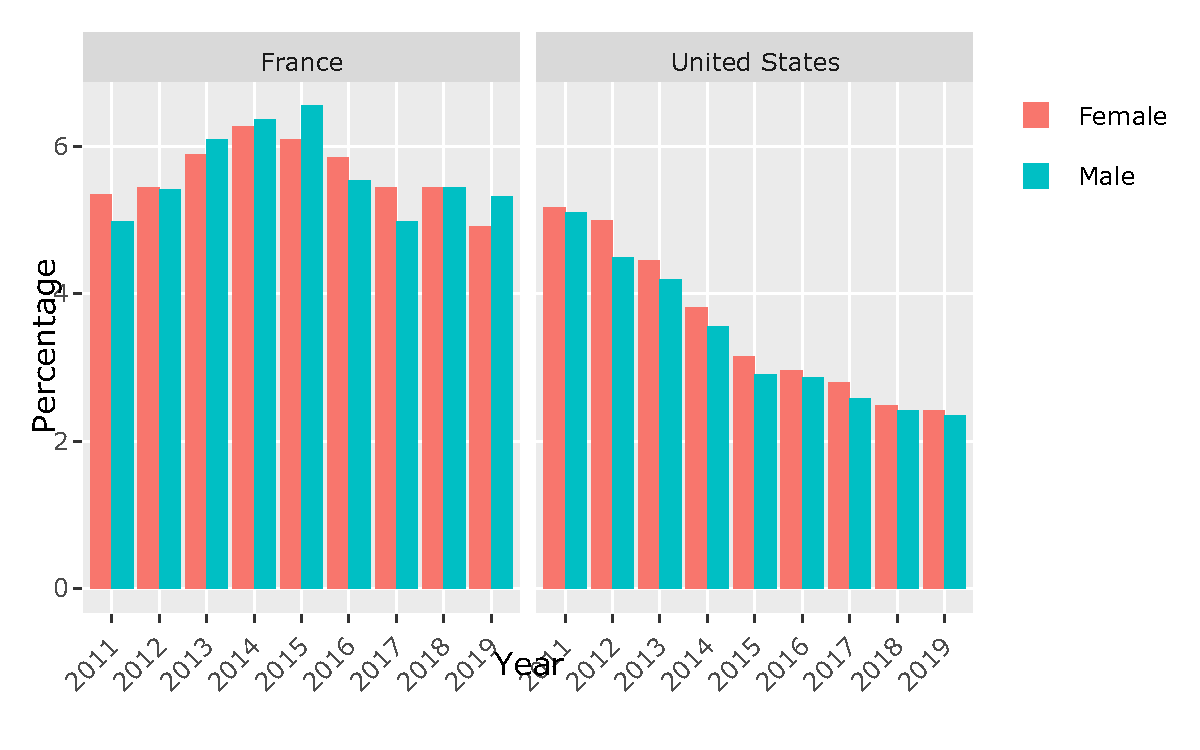
\includegraphics{The_Outsiders_5513_files/figure-latex/Advancedeved-1.pdf}
\caption{\label{fig:Advancedeved}Unemployment with advanced education in developed countries}
\end{figure}

Figure \ref{fig:Advancedeved} shows the unemployment percentage of males and females with advanced education in developed countries like United states and France.

\begin{figure}
\centering
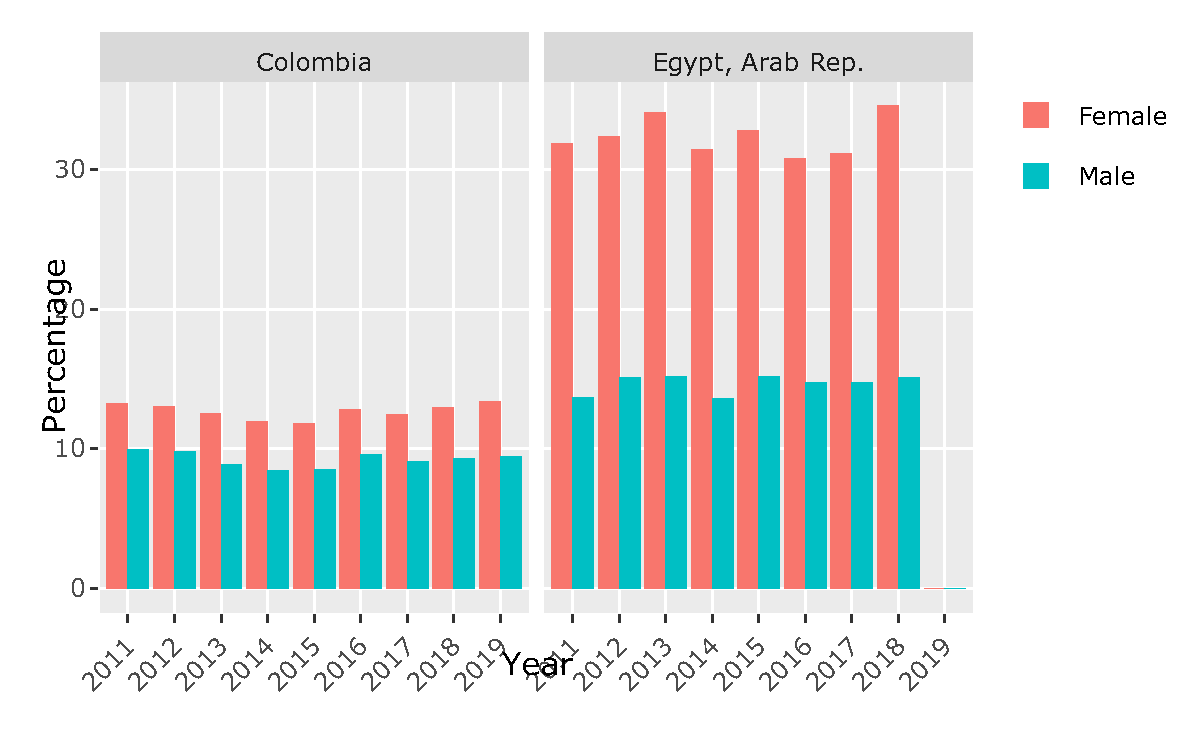
\includegraphics{The_Outsiders_5513_files/figure-latex/Advancedeving-1.pdf}
\caption{\label{fig:Advancedeving}Unemployment with advanced education in developing countries}
\end{figure}

Figure \ref{fig:Advancedeving} shows the unemployment percentage of males and females with advanced education in developing countries like Colombia and Egypt.

\begin{itemize}
\item
  Unemployment rates fall with higher educational attainment. As shown in figures \ref{fig:Advancedeved} and \ref{fig:Advancedeving} we can see that the overall percentage of unemployment is between 2\% to 6\% in developed countries and close to 10\% in developing countries.
\item
  Moreover the difference between the ratio of males and females unemployed is also low with advanced education for all countries except Egypt, where the difference is close to 15\%. Possible reasons for that include the high cost of childcare, the expectation that women carry out the majority of household responsibilities, negative attitudes toward women in the workplace, lack of mobility, legal barriers, persistent wage gaps, sexual harassment in the workplace, and poor enforcement of anti-discrimination laws \autocite{barriersegypt}
\end{itemize}

\clearpage

\textbf{Basic Education}

\begin{figure}
\centering
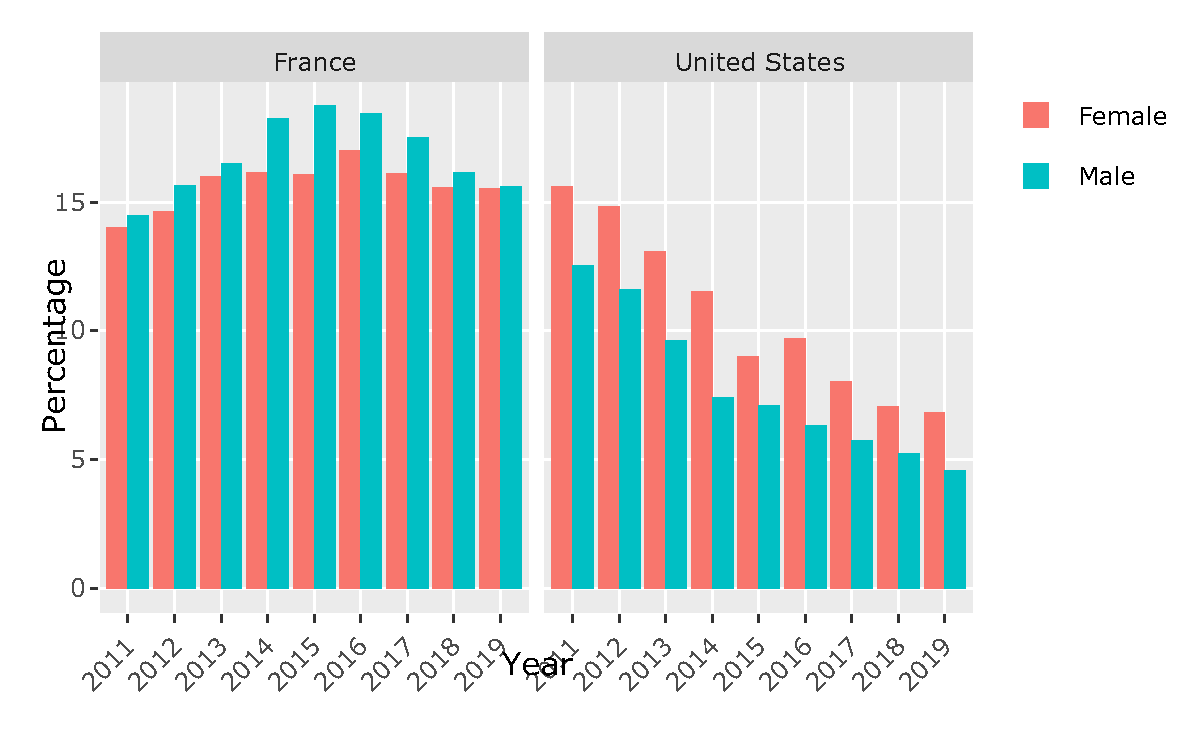
\includegraphics{The_Outsiders_5513_files/figure-latex/Basicdeved-1.pdf}
\caption{\label{fig:Basicdeved}Unemployment with basic education in developed countries}
\end{figure}

Figure \ref{fig:Basicdeved} shows the unemployment percentage of males and females with basic education in developed countries like United states and France.

\begin{figure}
\centering
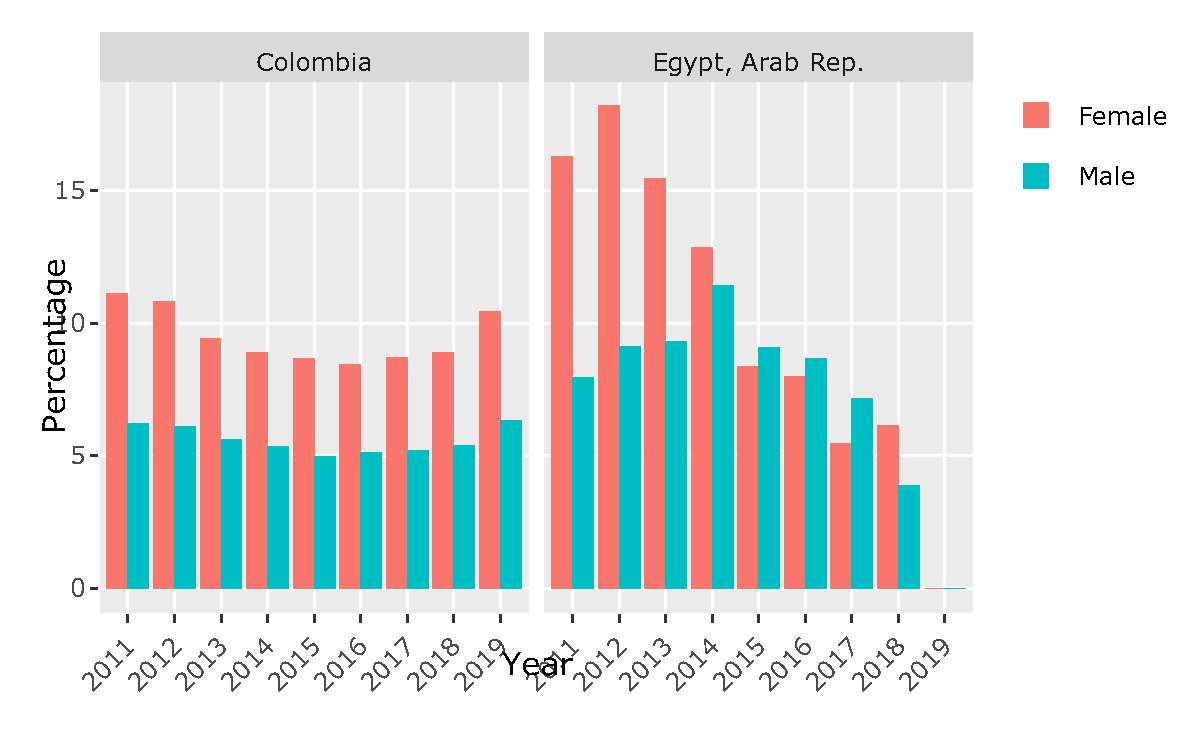
\includegraphics{The_Outsiders_5513_files/figure-latex/Basicdeving-1.pdf}
\caption{\label{fig:Basicdeving}Unemployment with basic education in developing countries}
\end{figure}

Figure \ref{fig:Basicdeving} shows the unemployment percentage of males and females with basic education in developing countries like Colombia and Egypt.

\begin{itemize}
\item
  It is interesting to see that the percentage of unemployment of males is more than that of females for all the years in France \ref{fig:Basicdeved}.
\item
  Figure \ref{fig:Basicdeving} Egypt shows that with just basic education the percentage of unemployment can decrease. The gap between males and females unemployment has gone down from 9\% to almost 3\% over the years.
\end{itemize}

\clearpage

\textbf{Intermediate Education}

\begin{figure}
\centering
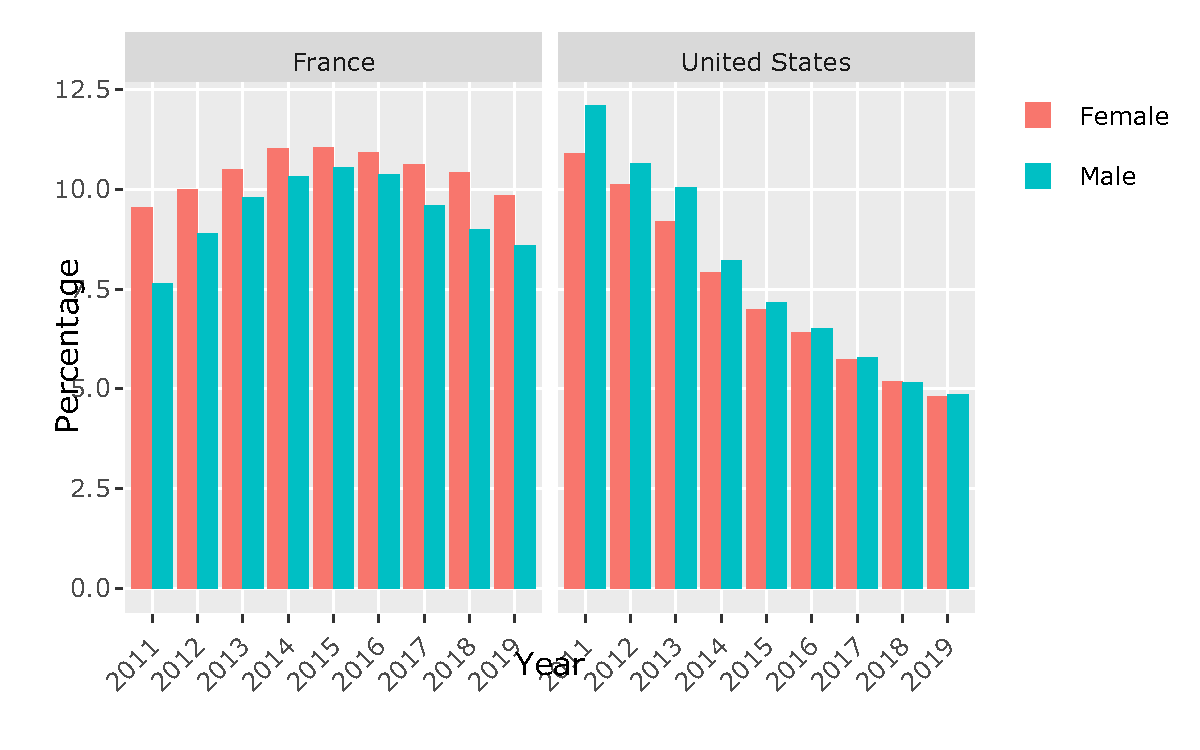
\includegraphics{The_Outsiders_5513_files/figure-latex/Intermediatedeved-1.pdf}
\caption{\label{fig:Intermediatedeved}Unemployment with intermediate education in developed countries}
\end{figure}

Figure \ref{fig:Intermediatedeved} shows the unemployment percentage of males and females with intermediate education in developed countries like United states and France.

\begin{figure}
\centering
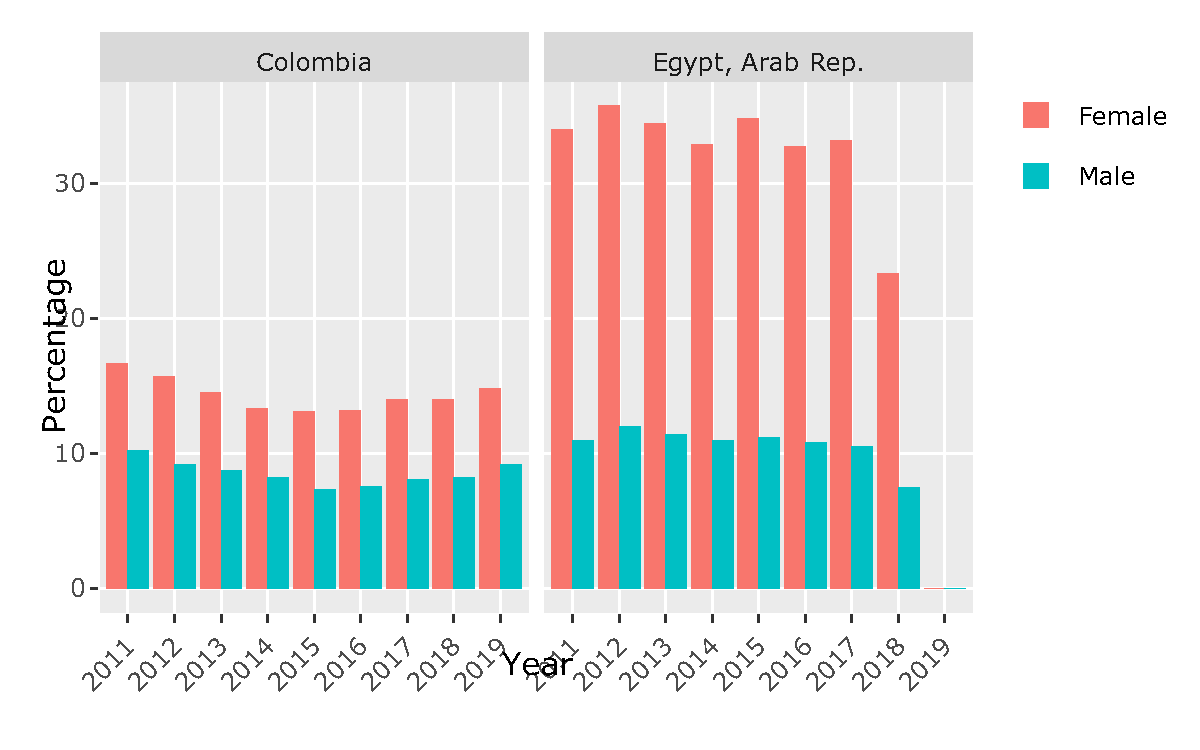
\includegraphics{The_Outsiders_5513_files/figure-latex/Intermediatedeving-1.pdf}
\caption{\label{fig:Intermediatedeving}Unemployment with intermediate education in developing countries}
\end{figure}

Figure \ref{fig:Intermediatedeving} shows the unemployment percentage of males and females with intermediate education in developing countries like Colombia and Egypt.

\begin{itemize}
\item
  Those with low educational attainment \textbf{intermediate education} are both less likely to be labor force participants and more likely to be unemployed. The greatest gender differences in unemployment rates are seen among adults with lower levels of education as shown in figure \ref{fig:Intermediatedeving}. The percentage of female unemployment is close to 30\% in females whereas its 11\% for males
\item
  Whereas in developed countries even though the percentage of unemployment is high with intermediate education, its satisfying to see that it is almost equal for both males and females \ref{fig:Intermediatedeved}. \autocite{education}
\end{itemize}

\clearpage

\hypertarget{conclusion}{%
\section{Conclusion}\label{conclusion}}

With the help of our analysis, we can conclude that even though the gap between males and females is reducing in developed countries in terms of employment, it is important that equal opportunities are given to the female gender in the developing countries as well. As with this many developing countries would also see their average annual GDP growth increase.

In regards of the employment in high and low income countries, it can be seen that females are always leading the services sector and in the case of males, industry and agriculture take the highest number of workers. But overall, the highest income level, the lowest the amount of people working in industries such as industry or agriculture.

\printbibliography

\end{document}
